\documentclass{article}
\usepackage[utf8]{inputenc}
\usepackage[a4paper, margin=2.5cm]{geometry}
\usepackage{graphicx} 
\usepackage{natbib}
\usepackage[french]{babel}

%\usepackage[default,scale=0.95]{opensans}
\usepackage[T1]{fontenc}
\usepackage{amssymb} %math
\usepackage{amsmath}
\usepackage{amsthm}
\usepackage{systeme}
\usepackage{bbm}
\usepackage{media9}
\usepackage{makecell}
\usepackage{url}
\usepackage{minted}
\usepackage{xcolor}
\usepackage{wrapfig}
\usepackage{csquotes}
\usepackage{subcaption}
\usepackage{float}
\usepackage{dirtree}

% \usepackage{lineno}
% \linenumbers

\usepackage{hyperref}
\hypersetup{
    % colorlinks=true,
    % linkcolor=blue,
    % filecolor=magenta,      
    % urlcolor=cyan,
    pdftitle={Projet ML},
    %pdfpagemode=FullScreen,
    }
\urlstyle{same} %\href{url}{Text}

\renewcommand{\baselinestretch}{1.5}
\graphicspath{{./src/}}

\begin{document}

\begin{titlepage}
    \begin{center}
        \vspace*{1cm}

        \Huge
        \textbf{ML - Projet}

        %\vspace{0.5cm}
        \LARGE
        Réseau de neurones from scratch

        %\vspace{1.5cm}
        \Large
        Charles \textsc{Vin}, Aymeric \textsc{Delefosse}

        \vfill
        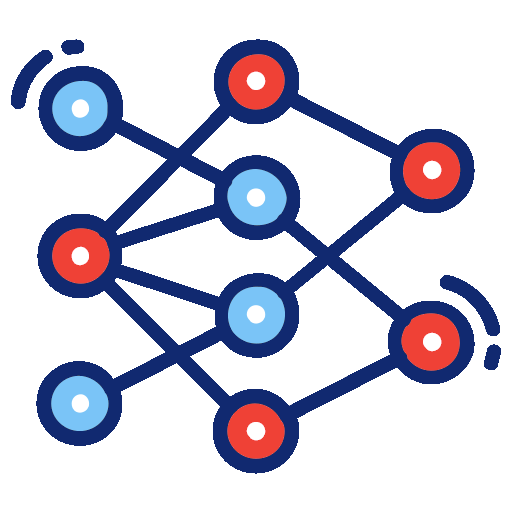
\includegraphics[width=.5\textwidth]{neural-network.png}    
        \vfill

        \large
        DAC | 2022-2023 \hfill 
        
\includegraphics[width=0.30\textwidth]{logo.png}
        \hfill
        
        
    \end{center}
\end{titlepage}

\tableofcontents
\newpage

\section{Introduction}

\section{Implémentation}

Le code est disponible sur \href{https://github.com/dataymeric/NeuralNetworksDIY}{ce dépôt GitHub}.

\begin{itemize}
    \item Implémentation optimisée de la convolution avec le moins de boucles possibles (utilisation de fonctions avancées de \texttt{numpy}); 
    \item Une documentation en ligne ;
    \item Implémentation d'un \texttt{logger} qui peut afficher graphiquement la \textit{loss} après chaque époque ; 
    \item Early stopping qui permet de réduire les temps d'apprentissage et les risques de sur-apprentissage.
\end{itemize}

La bibliothèque est organisée de manière analogue aux bibliothèques de \textit{deep learning} plus populaires.

\section{Expérimentation}

Dans le but de mettre notre bibliothèque à l'épreuve, nous avons entrepris une série d'expérimentations en utilisant diverses architectures sur deux types de données distincts. Le premier ensemble de données était constitué de jeux aléatoires de données gaussiennes, présentant des caractéristiques linéairement séparables ou non, tels que le XOR ou le jeu d'échecs. Le second ensemble de données concernait la classification d'images sur deux jeux de données : un pour la reconnaissance de chiffres (le plus populaire : \texttt{MNIST}) et le deuxième, plus complexe, pour la reconnaissance de vêtements (\texttt{Fashion MNIST}).

\subsection{Classification}

\subsubsection{Effet de l'initialisation des paramètres}

Nous avons très vite constaté le rôle et l'impact de l'initialisation des paramètres sur les performances des réseaux de neurones. Cette initialisation peut paraître anodine à première vue mais joue un rôle crucial sur la performance et la significativité du modèle. \\
Une initialisation inadéquate peut entraîner des problèmes tels que la saturation des neurones, la divergence de l'apprentissage ou la stagnation dans des minima locaux. Une initialisation judicieuse peut quant à elle favoriser une convergence plus rapide et une meilleure généralisation des données. \\
Ainsi, l'optimisation des poids et des biais à l'initialisation constitue une étape cruciale dans la conception et l'entraînement des réseaux de neurones. Cette initialisation peut se faire en prenant en compte les spécificités de l'architecture et de la fonction d'activation.

Ainsi, pour les modules utilisant des paramètres (linéaire et convolution), il est possible d'initialiser les poids et biais de huit manières différentes :

\begin{itemize}
    \item Initialisation normale : les paramètres sont initialisés selon une loi normale centrée réduite : $ W, B \sim \mathcal{N}(0, 1) $ ;
    \item Initialisation uniforme : les paramètres sont initialisés selon une loi uniforme : $ W, B \sim \mathcal{U}(0, 1) $ ;
    \item Initialisation à 1 : très simpliste, tous les paramètres sont initialisés à 1 ;
    \item Initialisation à 0 : très simpliste, tous les paramètres sont initialisés à 0 ;
    \item Initialisation de Xavier (ou de Glorot) : cette méthode, développée par Xavier Glorot et Yoshua Bengio, ajuste les poids de manière à maintenir une variance constante tout au long du réseau, en fonction du nombre d'entrées et de sorties de chaque couche. Cela favorise une propagation efficace du signal. Il est possible d'initialiser selon une loi normale ou une loi uniforme, où $ \text{input} $ représente la taille de l'entrée dans le cadre d'un module linéaire, le nombre de canaux d'entrée dans le cadre d'une convolution et $ \text{output} $ représente la taille de la sortie dans le cadre d'un module linéaire, le nombre de canaux en sortie (le nombre de \textit{feature maps}) dans le cadre d'une convolution.
    \begin{itemize}
        \item Loi normale : $ W, B \sim \mathcal{N}(0, \, \sqrt[]{\frac{2}{\text{input} + \text{output}}}) $ ;
        \item Loi uniforme : $ W, B \sim \mathcal{U}(- \sqrt[]{\frac{6}{\text{input} + \text{output}}}, \, \sqrt[]{\frac{6}{\text{input} + \text{output}}}) $.
    \end{itemize}
    \item Initialisation de He (ou de Kaiming) : Cette méthode, développée par Kaiming He et al., est similaire à l'initialisation de Xavier, mais elle prend en compte la variance spécifique des fonctions d'activation asymétriques, telles que la fonction ReLU. Elle permet une initialisation adaptée aux architectures utilisant ces fonctions d'activation. 
    \begin{itemize}
        \item Loi normale : $ W, B \sim \mathcal{N}(0, \, \sqrt[]{\frac{2}{\text{input}}}) $ ;
        \item Loi uniforme : $ W, B \sim \mathcal{U}(- \sqrt[]{\frac{6}{\text{input}}}, \, \sqrt[]{\frac{6}{\text{input}}}) $.
    \end{itemize}
\end{itemize}

\textbf{Note} : pour le module linéaire, les biais sont initialisés par défaut tandis que pour la convolution, les biais sont désactivés par défaut (sauf indication contraire).

Pour déterminer en pratique l'effet de l'initialisation des paramètres, nous avons mis en place un réseau très simple qui classifie le jeu de données \textit{fashion-mnist}. Celui-ci est composé d'une couche linéaire prenant en entrée l'image entière et classifiant sur dix neurones en sortie. On représentera par la suite les réseaux sous la forme suivante \texttt{Linear(784, 10) $ \rightarrow $ Sigmoid()}.

\begin{figure}[htbp]
    \centering
    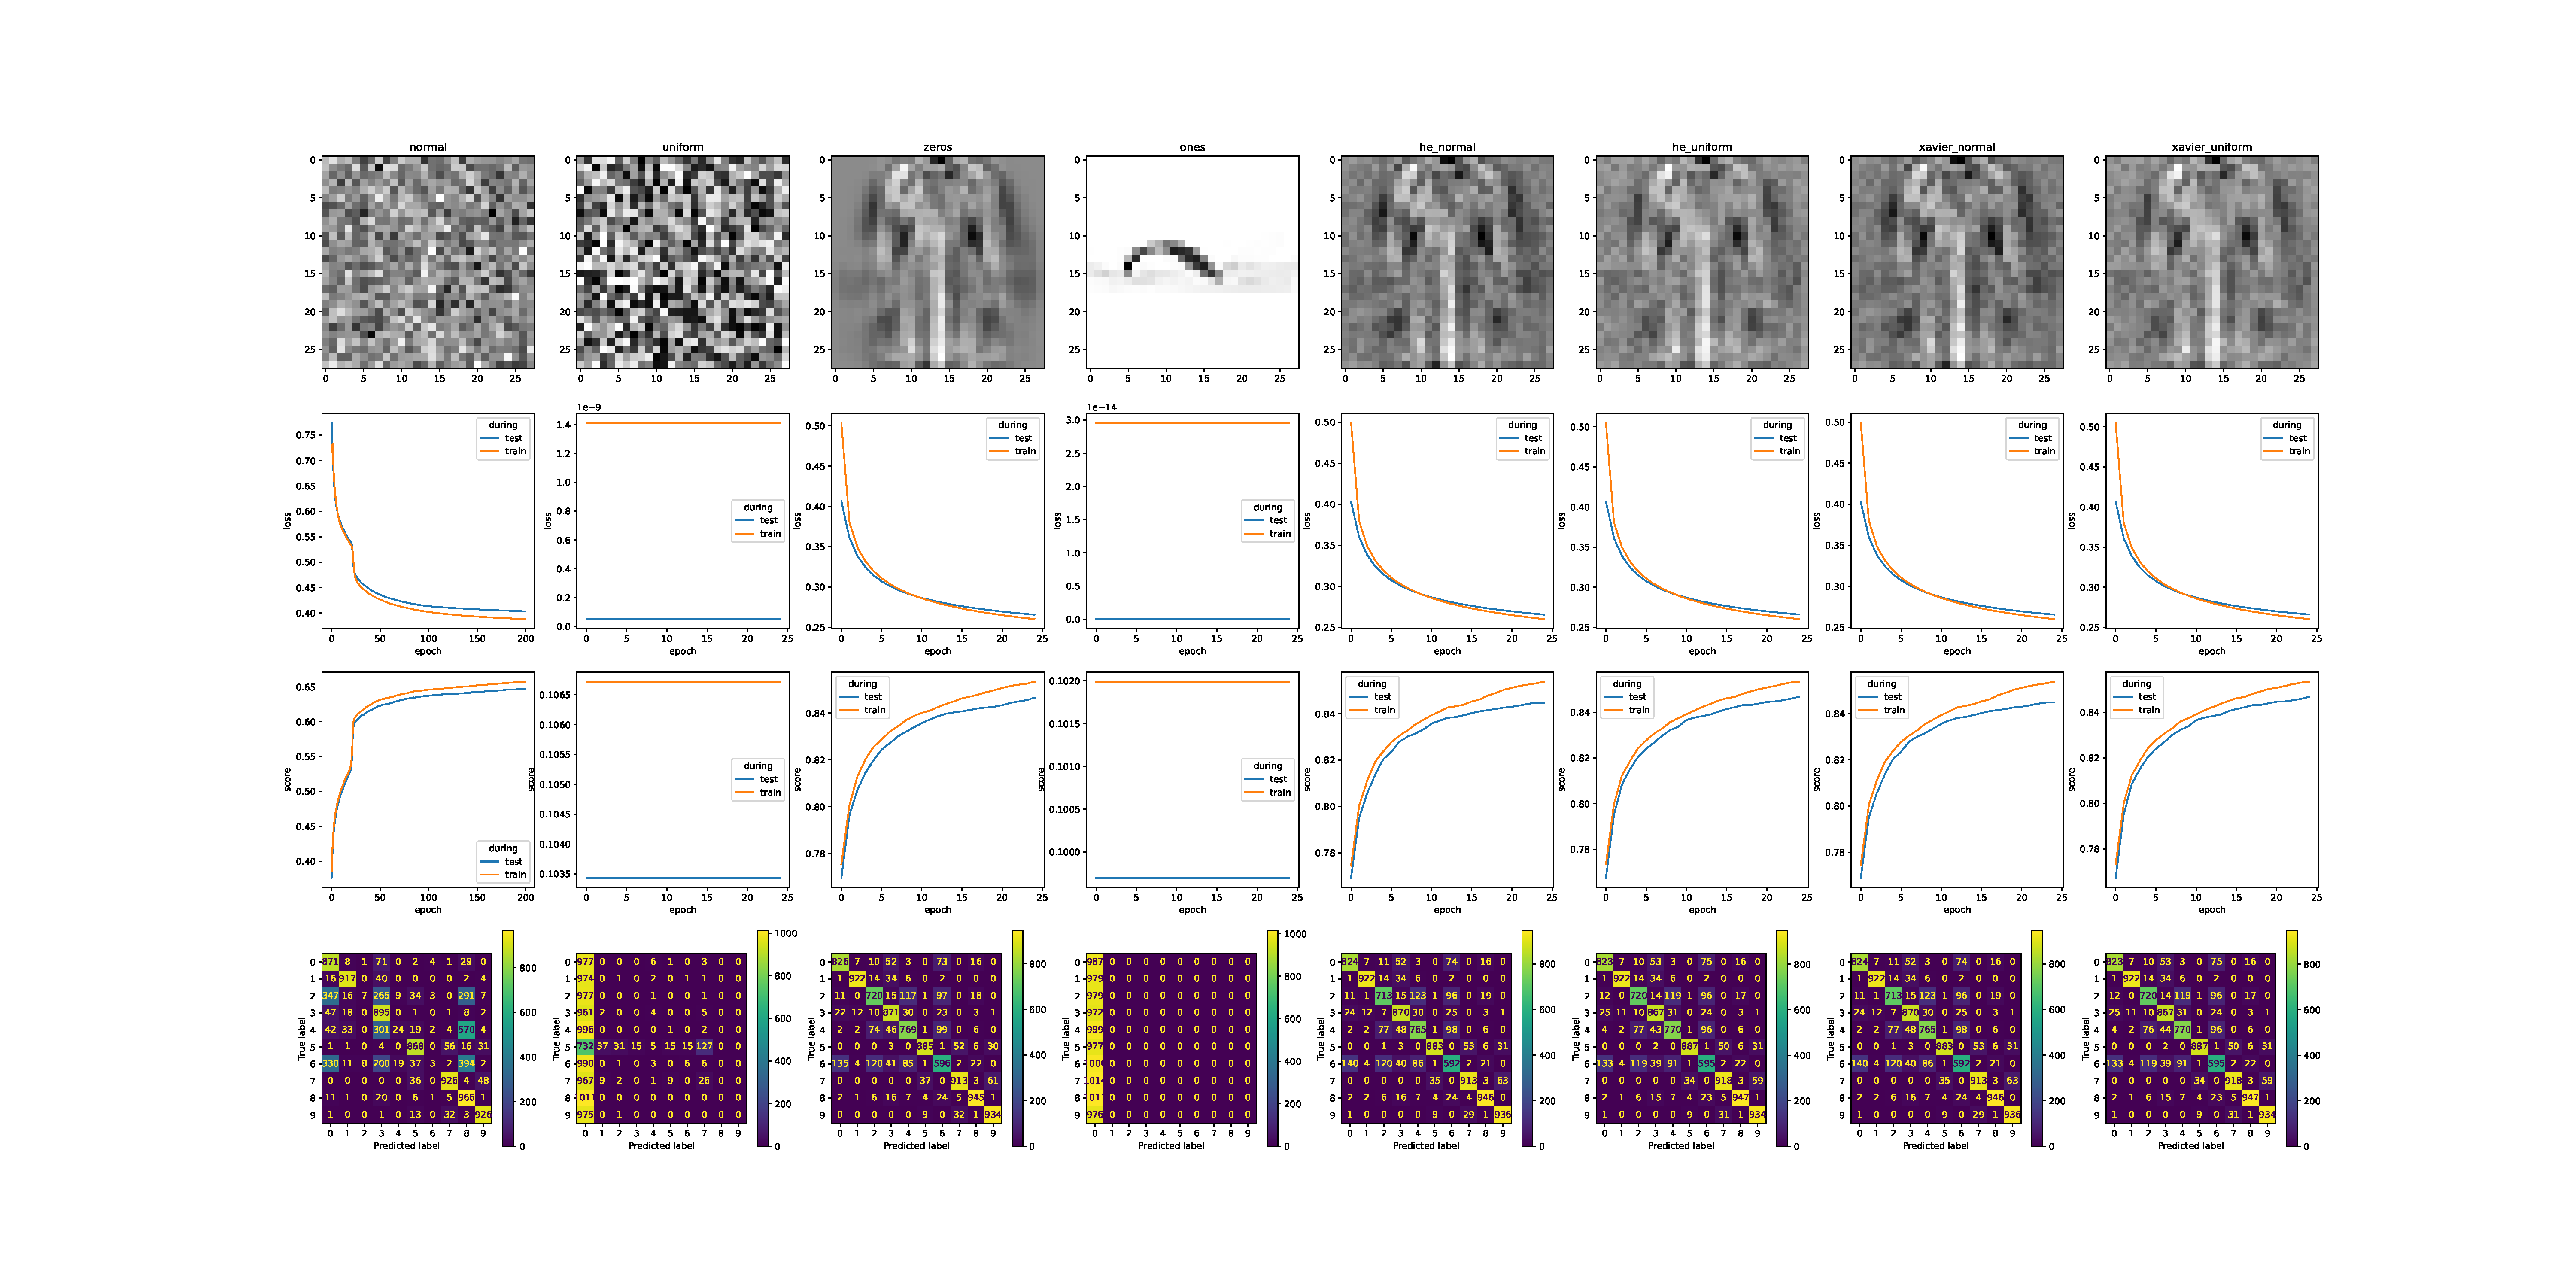
\includegraphics[width=\textwidth]{init_type.pdf}
    \caption{Représentation des paramètres, d'une matrice de confusion, de l'évolution du coût et du score par époque en fonction de l'initialisation des paramètres}
    \label{fig:initparam}
\end{figure}

La figure \ref{fig:initparam} représente les résultats de cette expérimentation. On constate des difficultés d'apprentissage sur certaines initialisations. L'initialisation normale tombe dans un minimum local (200 époques). Les initialisations uniforme et à 1 font exploser le gradient, empêchant tout apprentissage. 

Cette expérience a montrer l'impact important que peut avoir l'initialisation des paramètres. L'initialisation normale pourrait certainement être fixée en utilisant un autre algorithme d'optimisation, tel qu'Adam.

\subsubsection{Effet du taux d'apprentissage (\textit{learning rate})}

Le \textit{learning rate} est un hyperparamètre crucial dans l'entraînement des réseaux de neurones. Il contrôle la taille des pas que l'algorithme d'optimisation effectue lors de la mise à jour des poids du réseau pendant l'apprentissage. Un taux d'apprentissage adapté permet aux mises à jour de poids d'être suffisamment grandes pour converger rapidement vers un minimum, tout en évitant les oscillations et les divergences. Le but est donc de trouver un bon compromis entre la rapidité de convergence et la stabilité des résultats.

\begin{figure}[htbp]
    \centering
    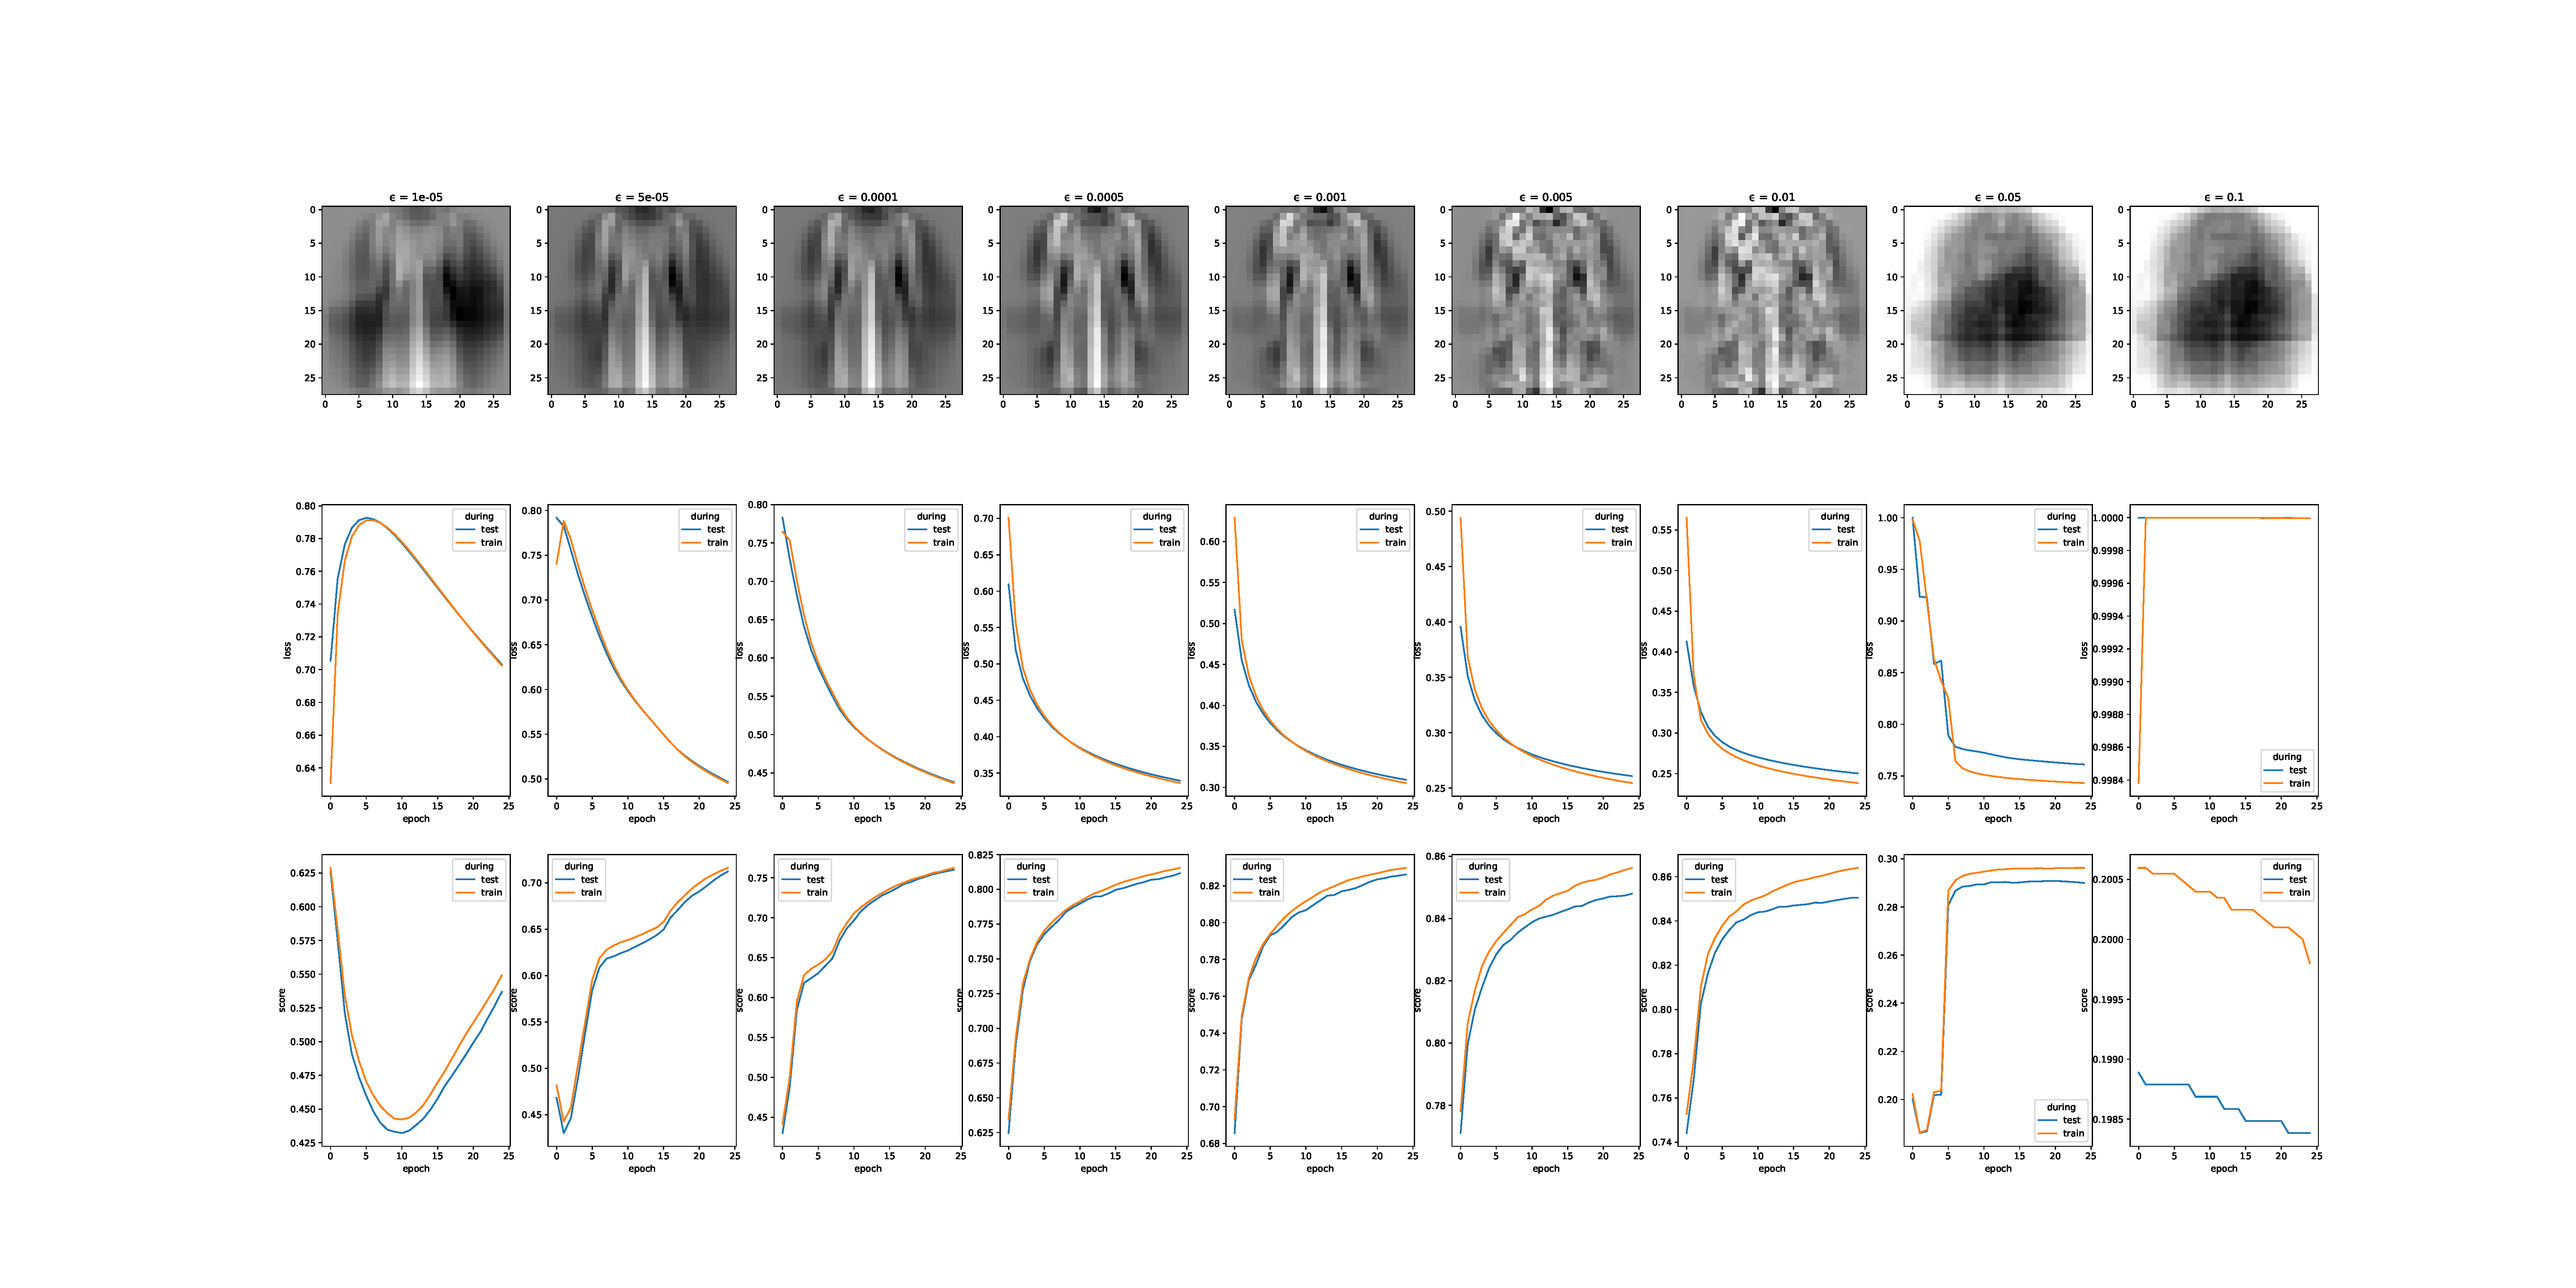
\includegraphics[width=\textwidth]{lr_effet.pdf}
    \caption{Représentation des paramètres, de l'évolution du coût et du score par époque en fonction du taux d'apprentissage $ \epsilon $ }
    \label{fig:effetlearningrate}
\end{figure}

Toujours avec le même réseau très simple, nous obtenons les résultats dans la figure \ref{fig:effetlearningrate}. 

Un \textit{learning rate} trop faible ralentit donc la convergence, et un nombre élevé d'itérations sera nécessaire pour atteindre une performance obtenue avec un taux d'apprentissage plus élevé. Les ajustements apportés aux poids sont également plus lents et progressifs, au risque de rester coincer dans des minima locaux peu optimaux.

Un \textit{learning rate} trop élevé entraîne une divergence dans notre cas, les poids se mettent à jour trop brutalement entraînant une convergence vers un modèle très rapidement sous-optimal.

\subsubsection{Effet des fonctions d'activation}

La fonction d'activation joue un rôle essentiel dans les réseaux de neurones : elle introduit une non-linéarité dans les activations du réseau, ce qui permet au modèle d'apprendre des représentations non linéaires complexes des données.

L'ajout d'une fonction d'activation non linéaire après un module linéaire, tel qu'une couche dense ou une convolution, permet d'introduire des interactions non linéaires entre les neurones et d'augmenter la capacité de représentation du modèle. Sans fonction d'activation, le réseau de neurones se réduirait simplement à une combinaison linéaire des entrées, limitant ainsi sa capacité à modéliser des relations complexes.

Différentes fonctions d'activation peuvent être utilisées en fonction du problème et des caractéristiques des données. Par exemple :

\begin{itemize}
    \item La fonction tangente hyperbolique qui comprime les sorties entre -1 et 1 ;
    \item La fonction sigmoïde qui comprime les sorties entre 0 et 1 ;
    \item La fonction sigmoïde "stable" qui a été implémentée dans l'optique d'éviter des instabilités numériques ;
    \item La fonction softmax pour transformer les données en une distribution de probabilités ;
    \item La fonction log-softmax afin d'éviter des instabilités numériques ;
    \item La fonction ReLU ;
    \item La fonction LeakyReLU afin d'éviter du \textit{gradient vanishing} et empêcher la rétropropagation du gradient ;
    \item La fonction SoftPlus qui est une autre approximation de la fonction ReLU.
\end{itemize}

On pourrait, rajouter encore d'autres fonctions d'activation, telles que la fonction identité, une identité courbée, une sinusoïde, un sinus cardinal, une fonction gaussienne...

Le choix de la fonction d'activation dépend du problème à résoudre, des caractéristiques des données et de l'architecture du réseau. Chaque fonction d'activation a des propriétés différentes et peut être plus adaptée à certains types de problèmes ou à certaines architectures.

\begin{figure}[htbp]
    \centering
    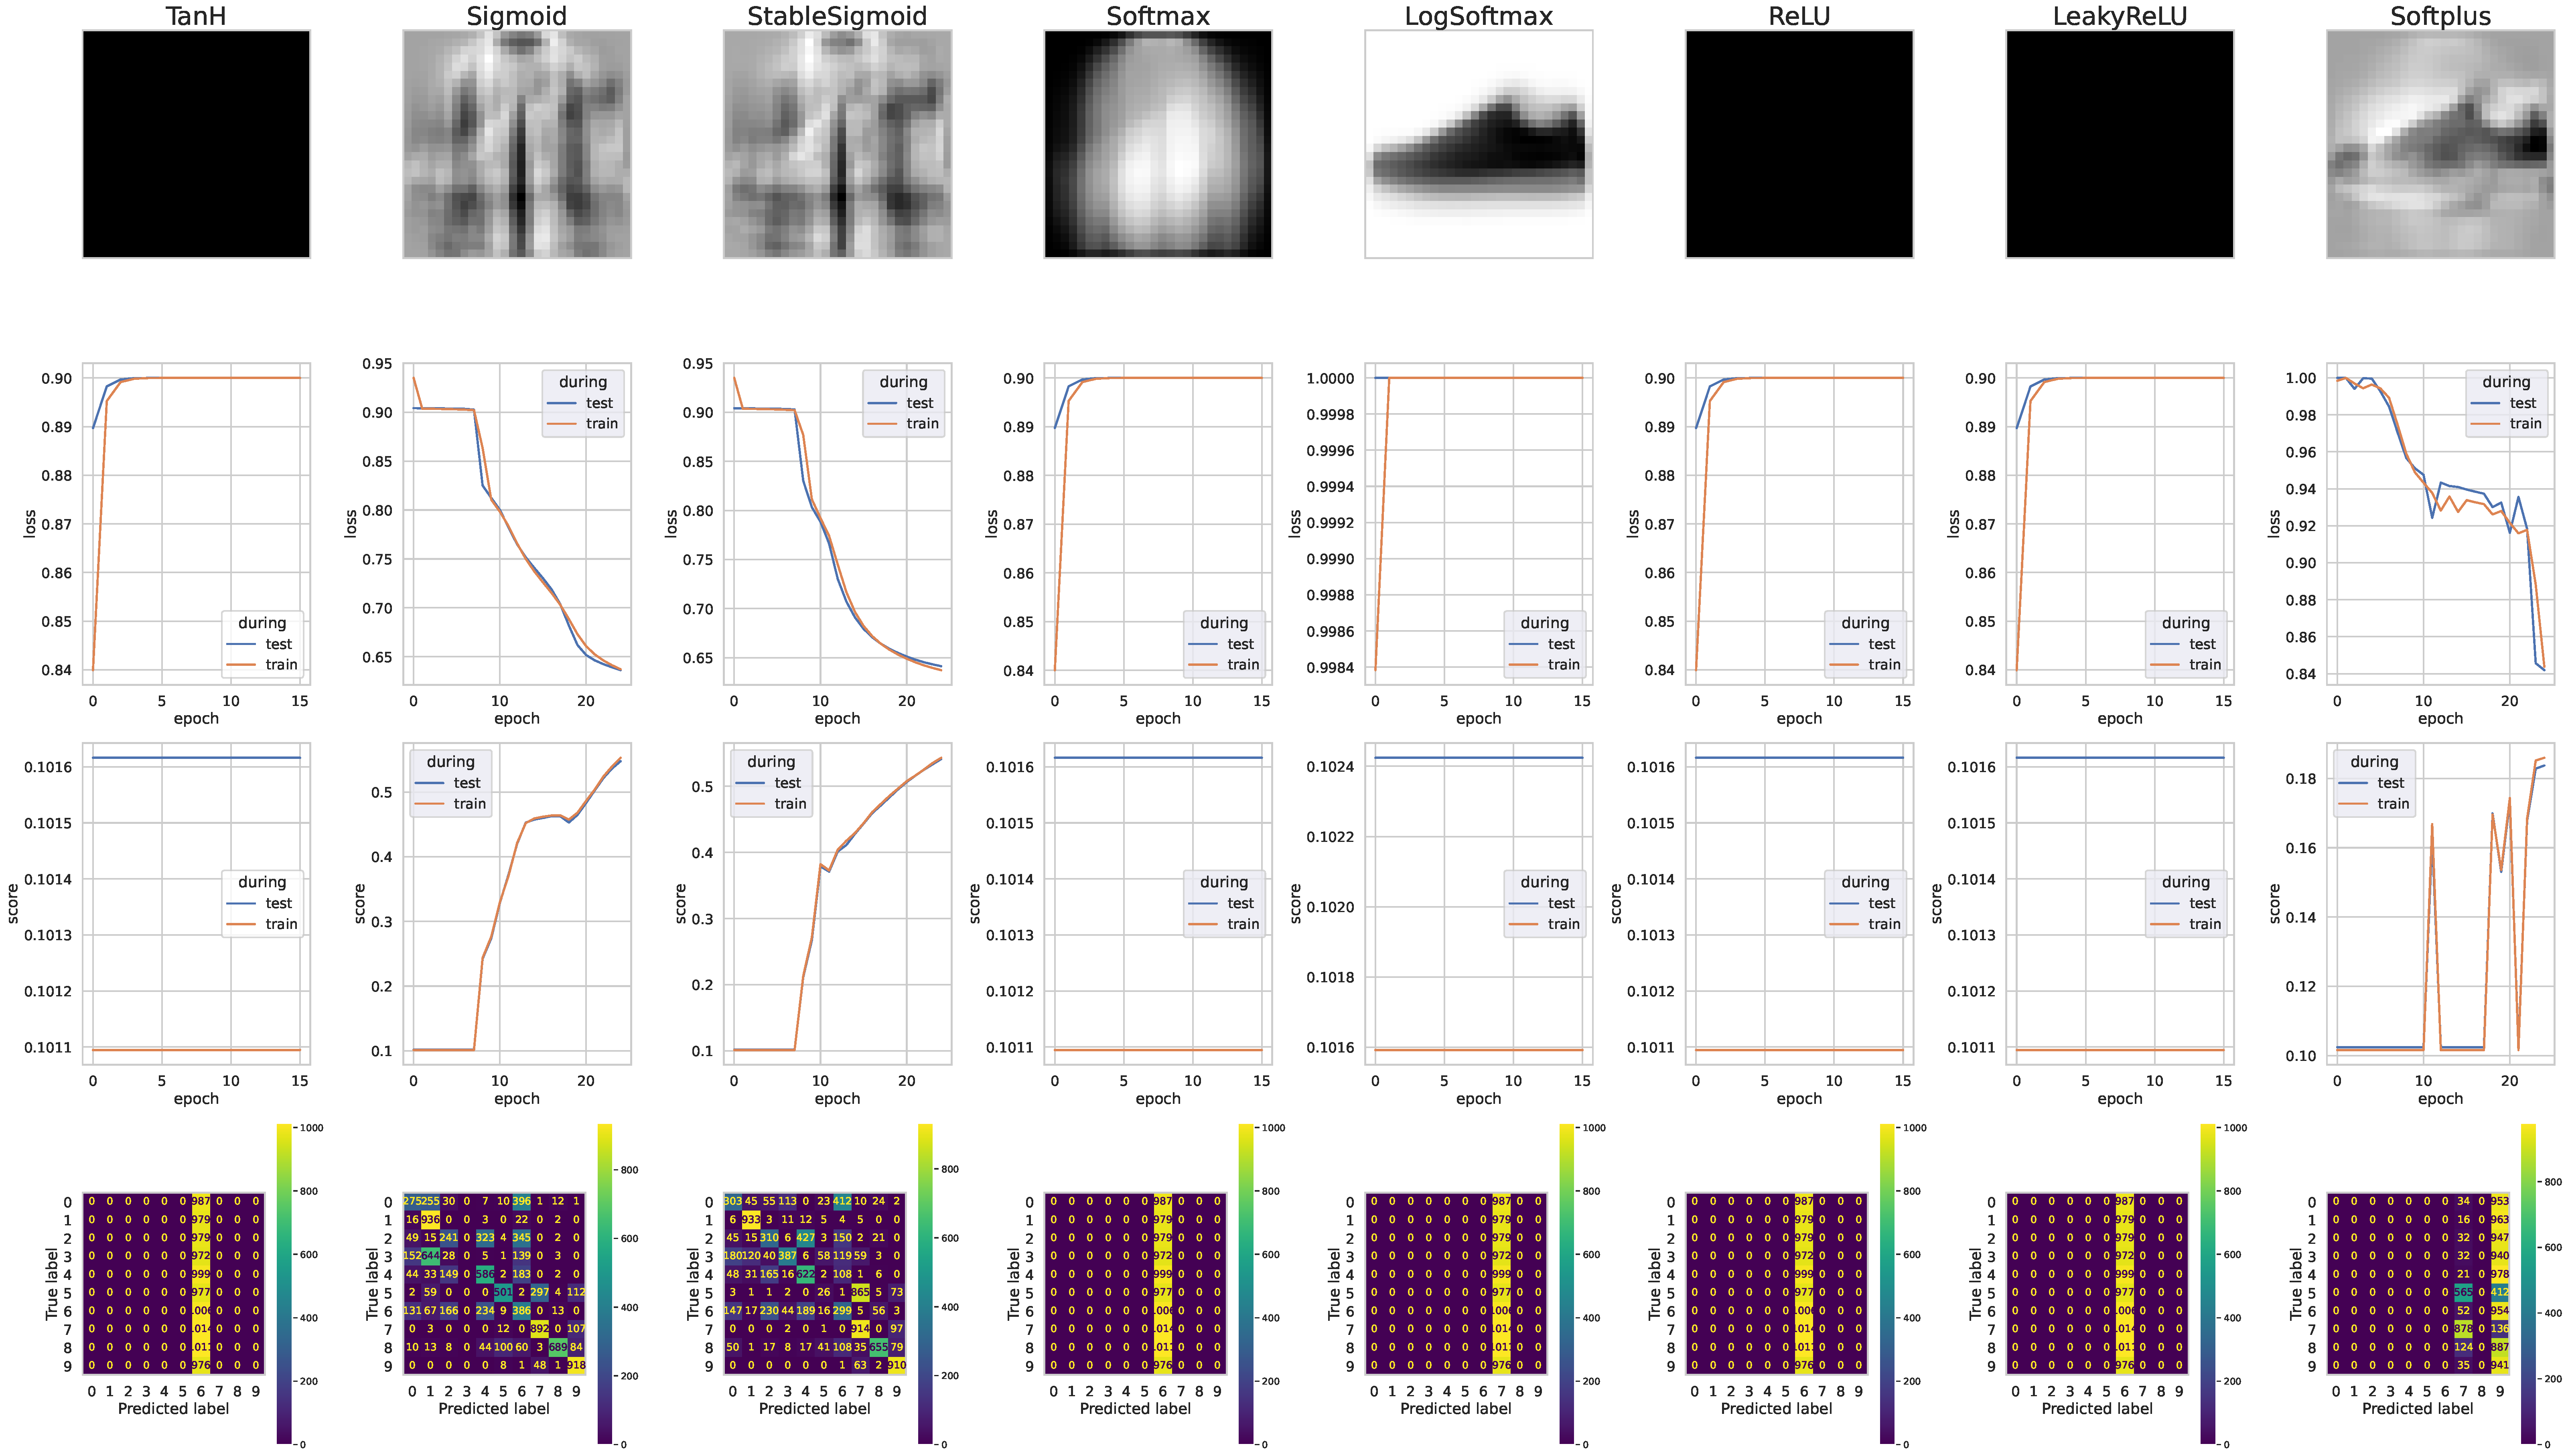
\includegraphics[width=\textwidth]{activation_func.pdf}
    \caption{Représentation des paramètres, de l'évolution du coût et du score par époque en fonction du taux d'apprentissage $ \epsilon $ }
    \label{fig:activationfunc}
\end{figure}

\subsection{Classification et convolution}

Même avec un multi-layer perceptron, on parvient à obtenir des performances correctes sur des images. Et si on utilisait des réseaux de neurones convolutifs ? L'intérêt de la convolution étant de capturer les motifs locaux, de réduire le nombre de paramètres à apprendre, d'obtenir une certaine invariance aux translations et de réduire la dimensionnalité des données, c'est un module particulièrement adapté aux images, aux séquences temporelles ou signaux.

La convolution en une dimension est implémentée et fonctionnelle, ainsi que les deux couches de pooling (Max et Average). Elles ont toutes été implémentées en utilisant le moins de boucles possibles afin d'avoir une implémentation la plus performante possible (seulement une boucle présente dans la convolution, sur la taille du kernel) grâce aux fonctions avancées de \texttt{numpy}. Le raisonnement a été détaillé au sein du code.

Un réseau utilisant une seule couche convolutionnelle de ce type \texttt{Conv1D(3,1,32) $\rightarrow$ MaxPool1D(2,2) $\rightarrow$ Flatten() $\rightarrow$ Linear(4064,100) $\rightarrow$ ReLU() $\rightarrow$ Linear(100,10)} fonctionne extrêmement bien dans le cadre de la reconnaissance de chiffres.

Sur une taille de batch fixée à 32, un nombre d'époques à 50 et un early-stopping à 5, répété 10 fois, on obtient un score en apprentissage de $ 99.36 \pm 0.0017\% $ et un score en évaluation de $ 97.08 \pm 0.0016 \% $, en $ 31 \pm 6 $ époques. 

Par ailleurs, l'initialisation est très importante dans les couches convolutionnelles, par exemple une initialisation des poids à zéros ne marche pas (figure \ref{fig:convinit}). Ici, les convolutions sont initialisées grâce à une initialisation de Xavier selon une loi normale et les modules linéaires grâce à une itialisation de He normale.

\begin{figure}[htbp]
    \centering
    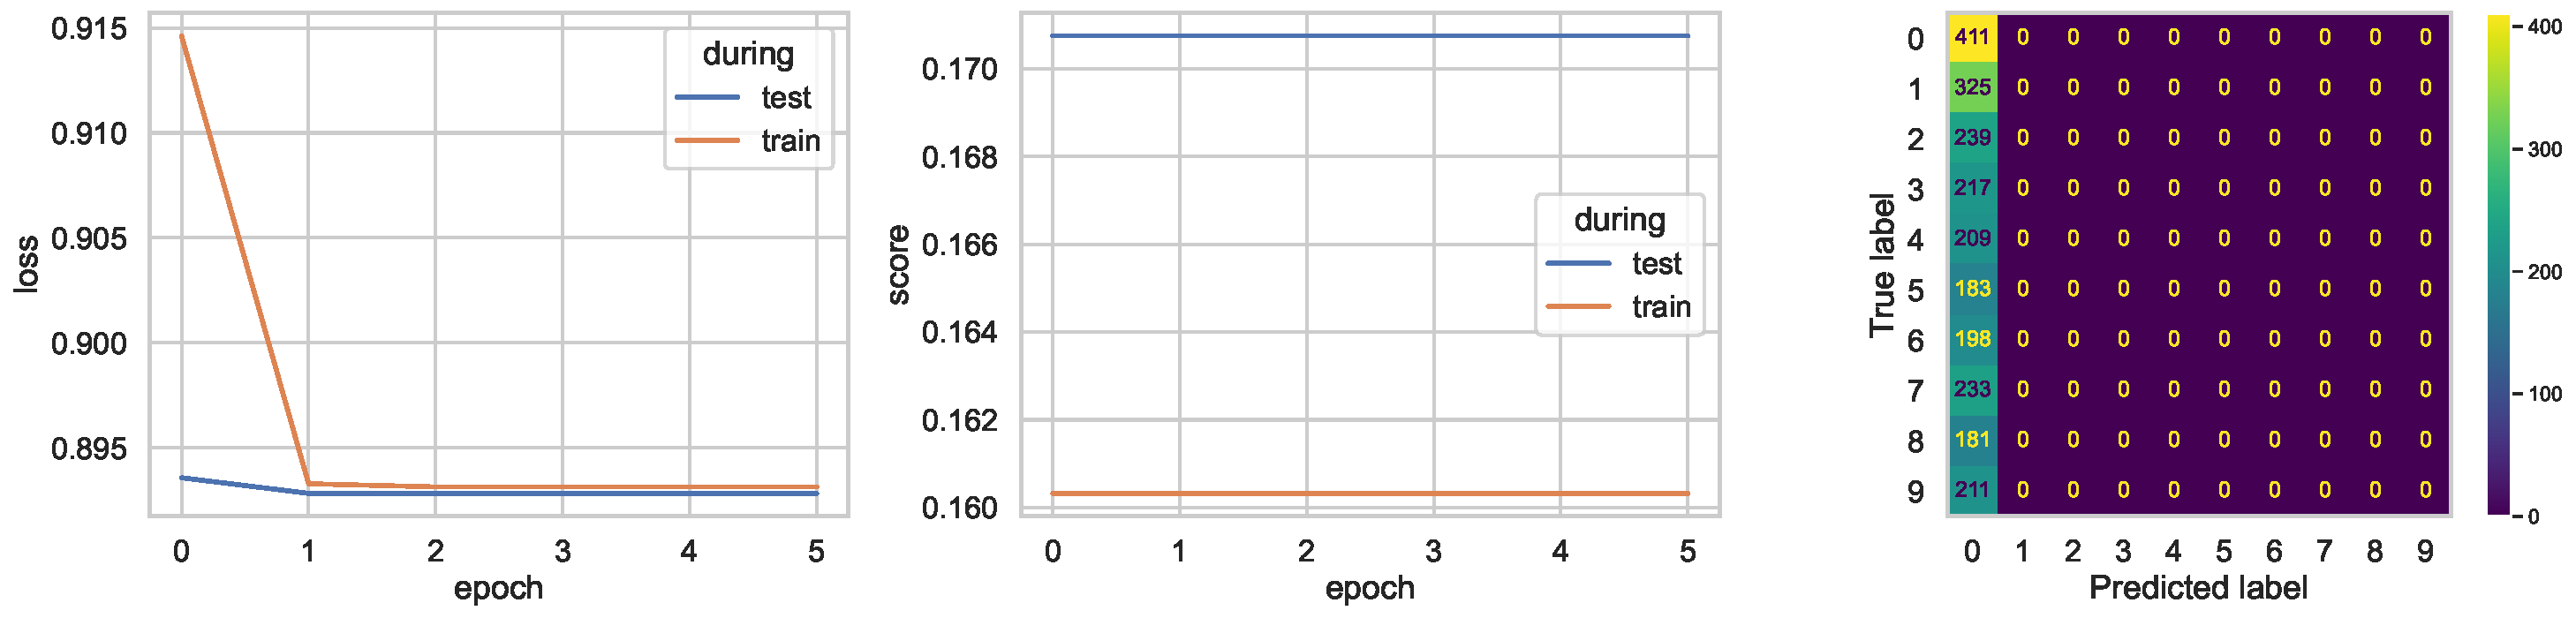
\includegraphics[width=\textwidth]{conv/conv_32batch_zeros.pdf}
    \caption{Impact de l'initialisation sur un réseau de neurones convolutionnel}
    \label{fig:convinit}
\end{figure}


\subsubsection{Effet de la taille des \textit{batch}}

Le nombre de batchs est un hyper-paramètre assez important de notre modèle. Ainsi, on obtient des meilleurs performances en apprenant sur des batchs plus petit, ce qui est courant et connu en \textit{deep learning}, mais s'apparente actuellement à du sur-apprentissage, même si l'on obtient des bons résultats en évaluation. De plus, plus la taille du batch sera petite, plus long sera l'apprentissage. Avec des batchs plus grand, le temps d'apprentissage sera très réduit mais les performances également ; sans compter que cela affecte également les instabilités numériques (explosion du gradient).

\subsubsection{Effet de la taille du kernel}

En faisant varier la taille du kernel, on se permet de capturer des motifs ou des informations de différentes échelles spatiales dans les données (ou non). Par exemple, des kernels de petite taille peuvent être efficaces pour détecter des détails fins, tandis que des kernels de plus grande taille peuvent être plus adaptés pour détecter des caractéristiques plus globales. Sur les données des chiffres manuscrits, les chiffres font partie intégrante de l'image, mais l'image est petite.

\begin{figure}[htbp]
    \centering
    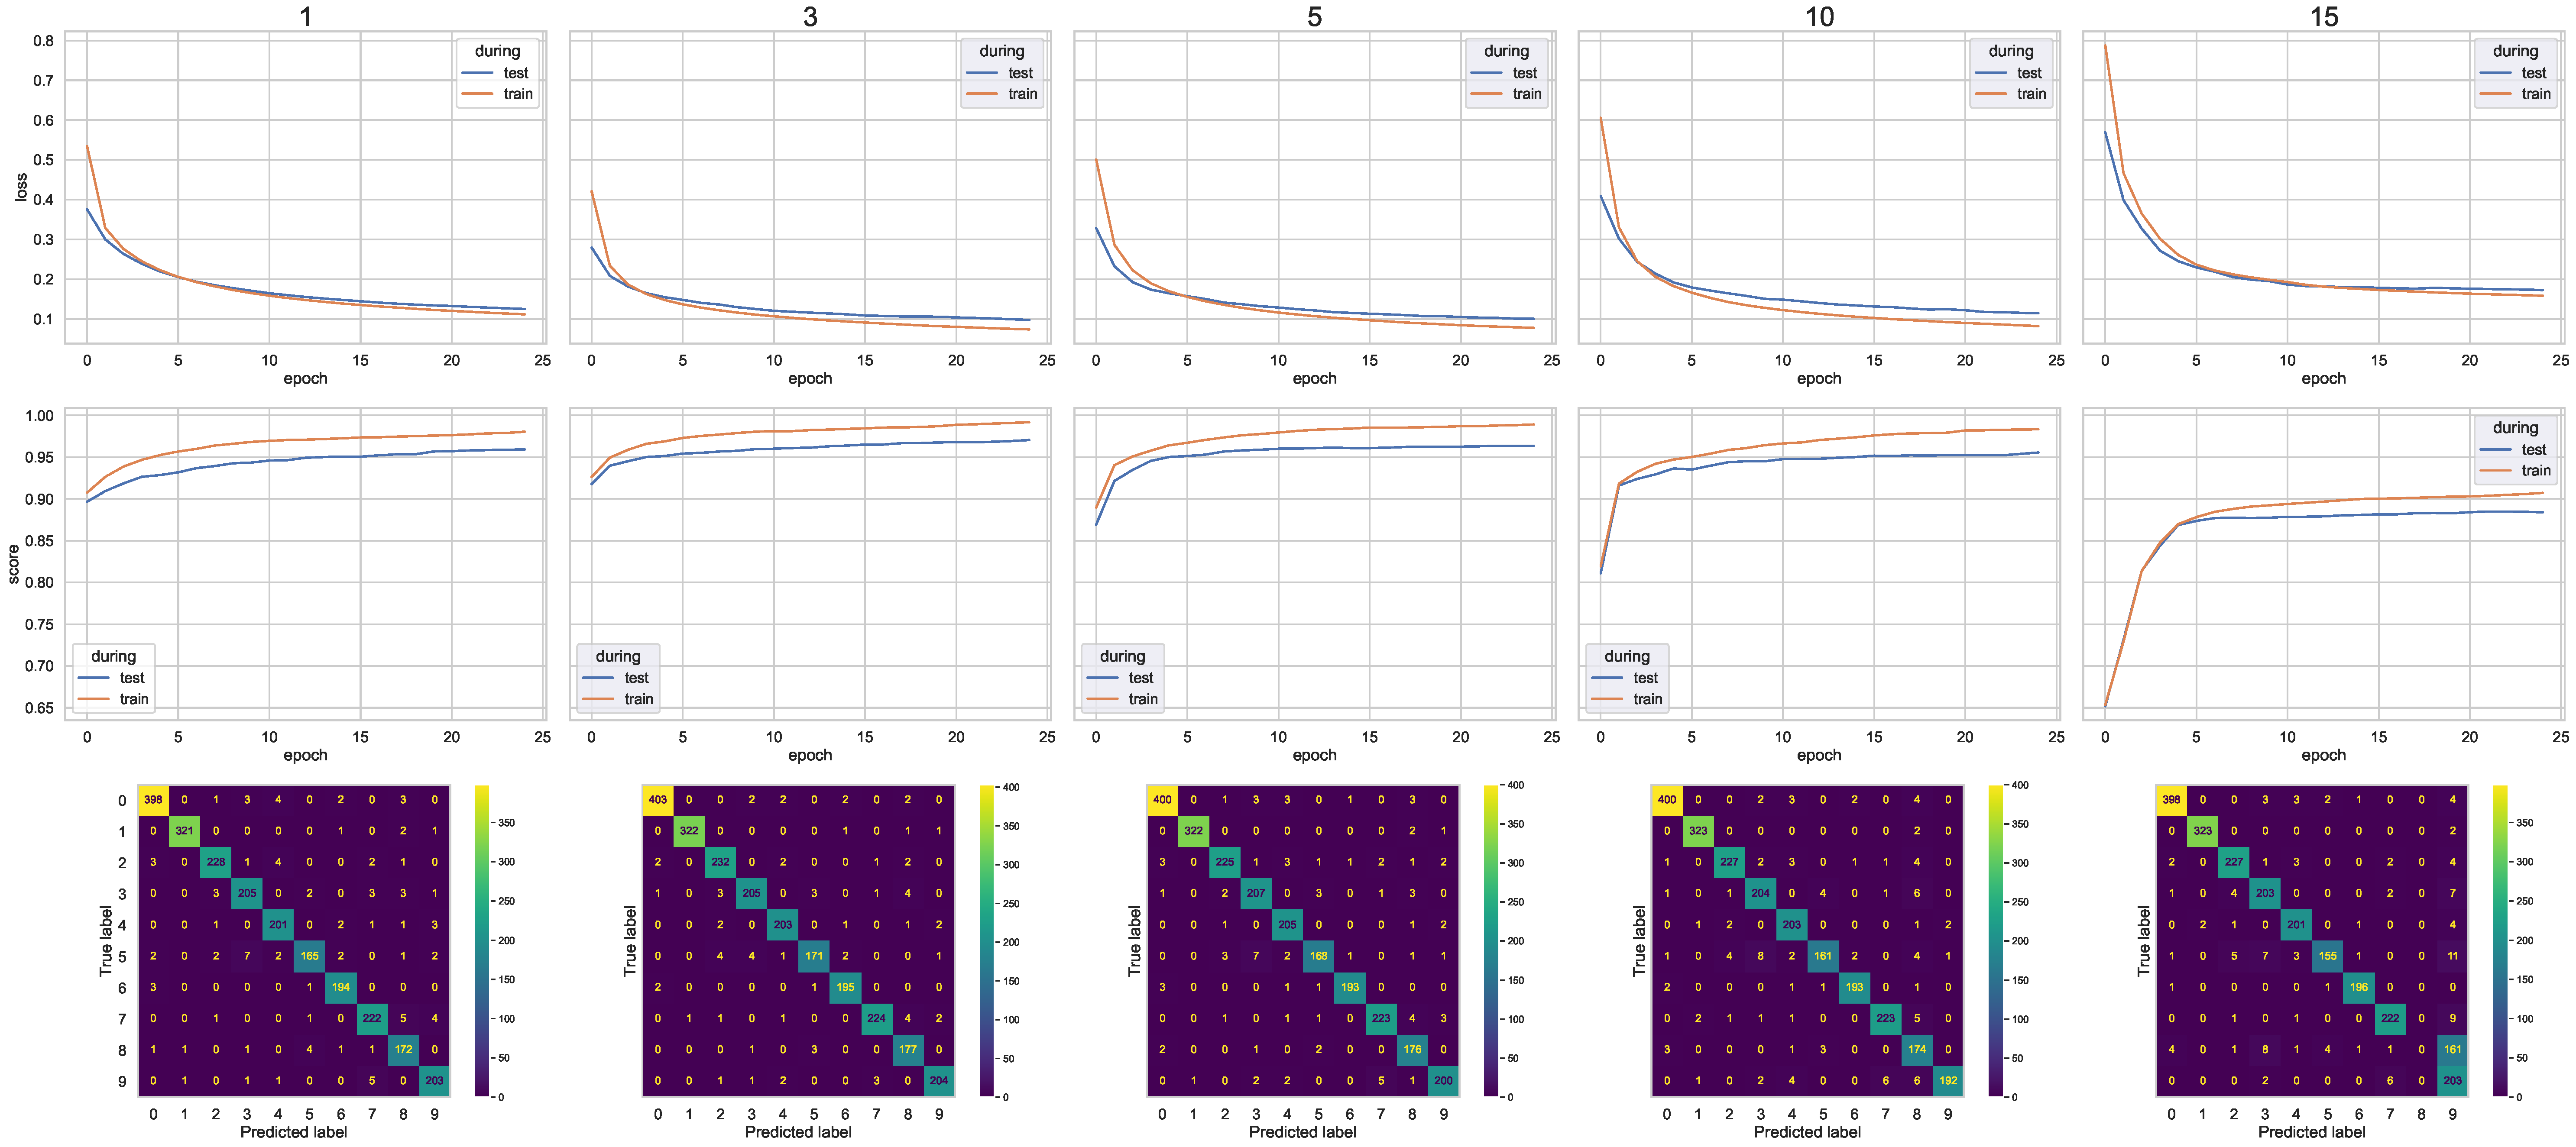
\includegraphics[width=\textwidth]{conv/conv_ksize.pdf}
    \caption{Impact de la taille du kernel pour un réseau de neurones convolutionnel}
    \label{fig:convksize}
\end{figure}

\subsubsection{Effet du nombre de \textit{feature maps}}

Le nombre de feature maps dans une couche de convolution influence la capacité du modèle à capturer des caractéristiques et des motifs complexes, améliorant ainsi la représentation des données et la capacité de généralisation. Cependant, il faut trouver un équilibre en tenant compte des contraintes de ressources et des exigences spécifiques du problème. 

\begin{figure}[htbp]
    \centering
    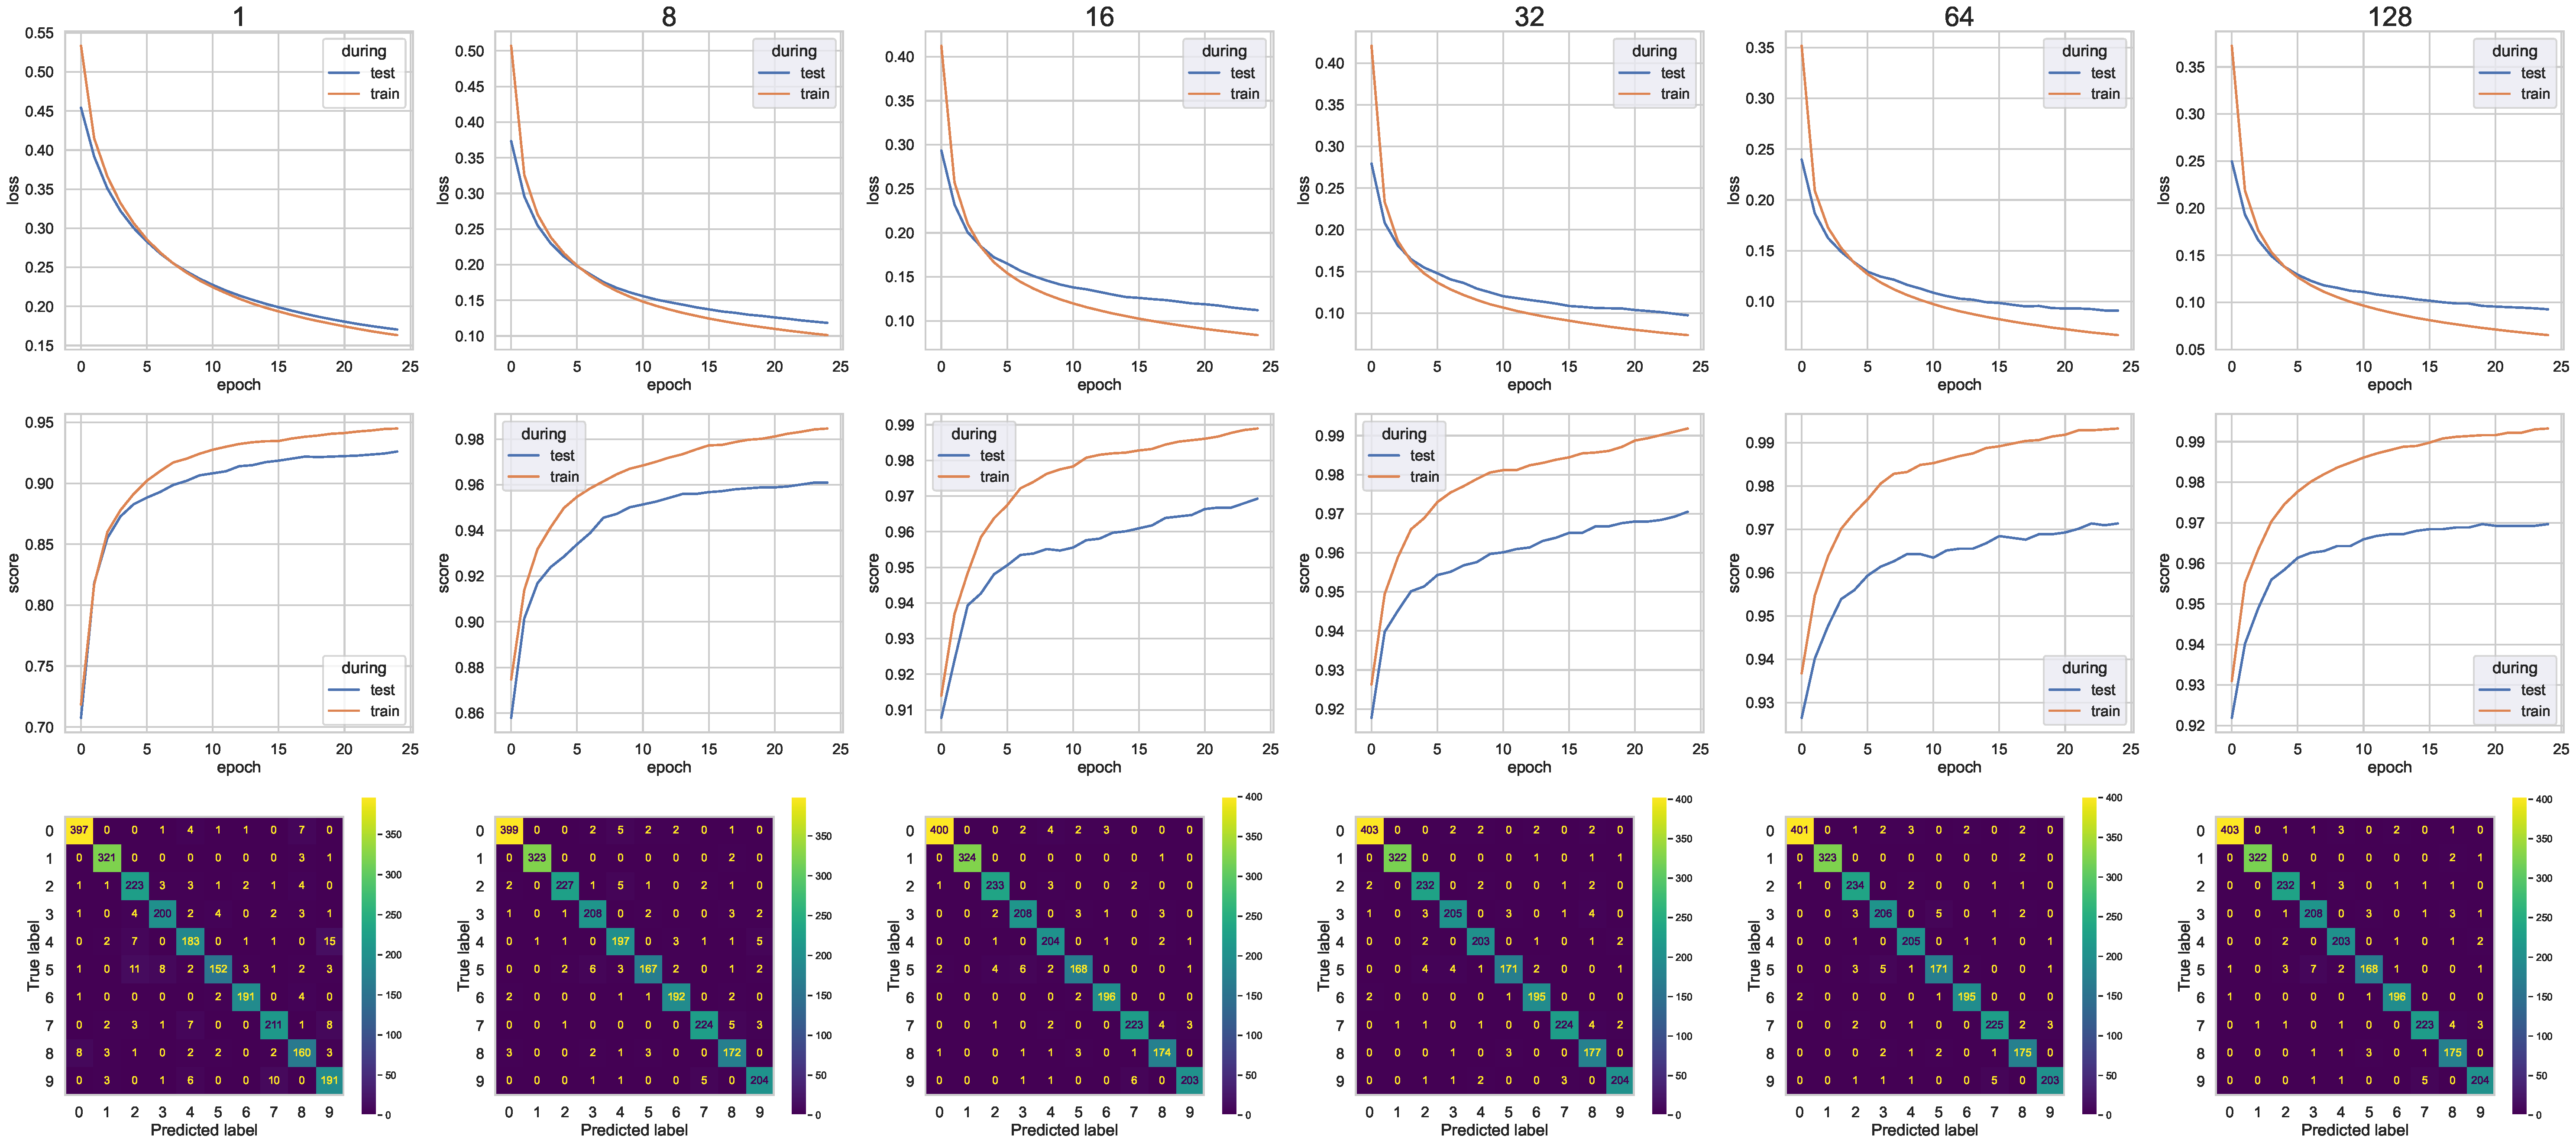
\includegraphics[width=\textwidth]{conv/conv_feature_maps.pdf}
    \caption{Impact du nombre de \textit{feature maps} pour un réseau de neurones convolutionnel}
    \label{fig:convchanout}
\end{figure}

\subsubsection{Diverses architectures}

Diverses architectures ont également été testées, pour voir la robustesse (ou non) de la convolution et sa capacité à surapprendre ou non, en particulier en agrandissant la profondeur des réseaux. Quelques variantes ont été utilisées en appliquant une fonction d'activation directement sur la convolution, ce qui est courant de faire, sans grand résultats. Finalement, un plus gros réseau convonlutionnel n'est pas synonyme de meilleure classification.

\paragraph*{Deux couches convolutionnelles} 

\texttt{Conv1D(3, 1, 32, 1)} $\rightarrow$ \texttt{ReLU()} $\rightarrow$ \texttt{MaxPool1D(2, 2)} $\rightarrow$
\texttt{Conv1D(3, 32, 32)} $\rightarrow$ \texttt{ReLU()} $\rightarrow$ \texttt{MaxPool1D(2, 2)} $\rightarrow$
\texttt{Flatten()} $\rightarrow$
\texttt{Linear(1984, 10)}

Les résultats sont sur la figure \ref*{fig:conv2layers} : les résultats ne sont pas catastrophiques, le réseau commence à apprendre, avant de subitement désapprendre. Les performances sont bien en-deça de celui du réseau précédent, avoir une couche linéaire n'est sûrement pas suffisante pour correctement classifier nos données.

\begin{figure}[htbp]
    \centering
    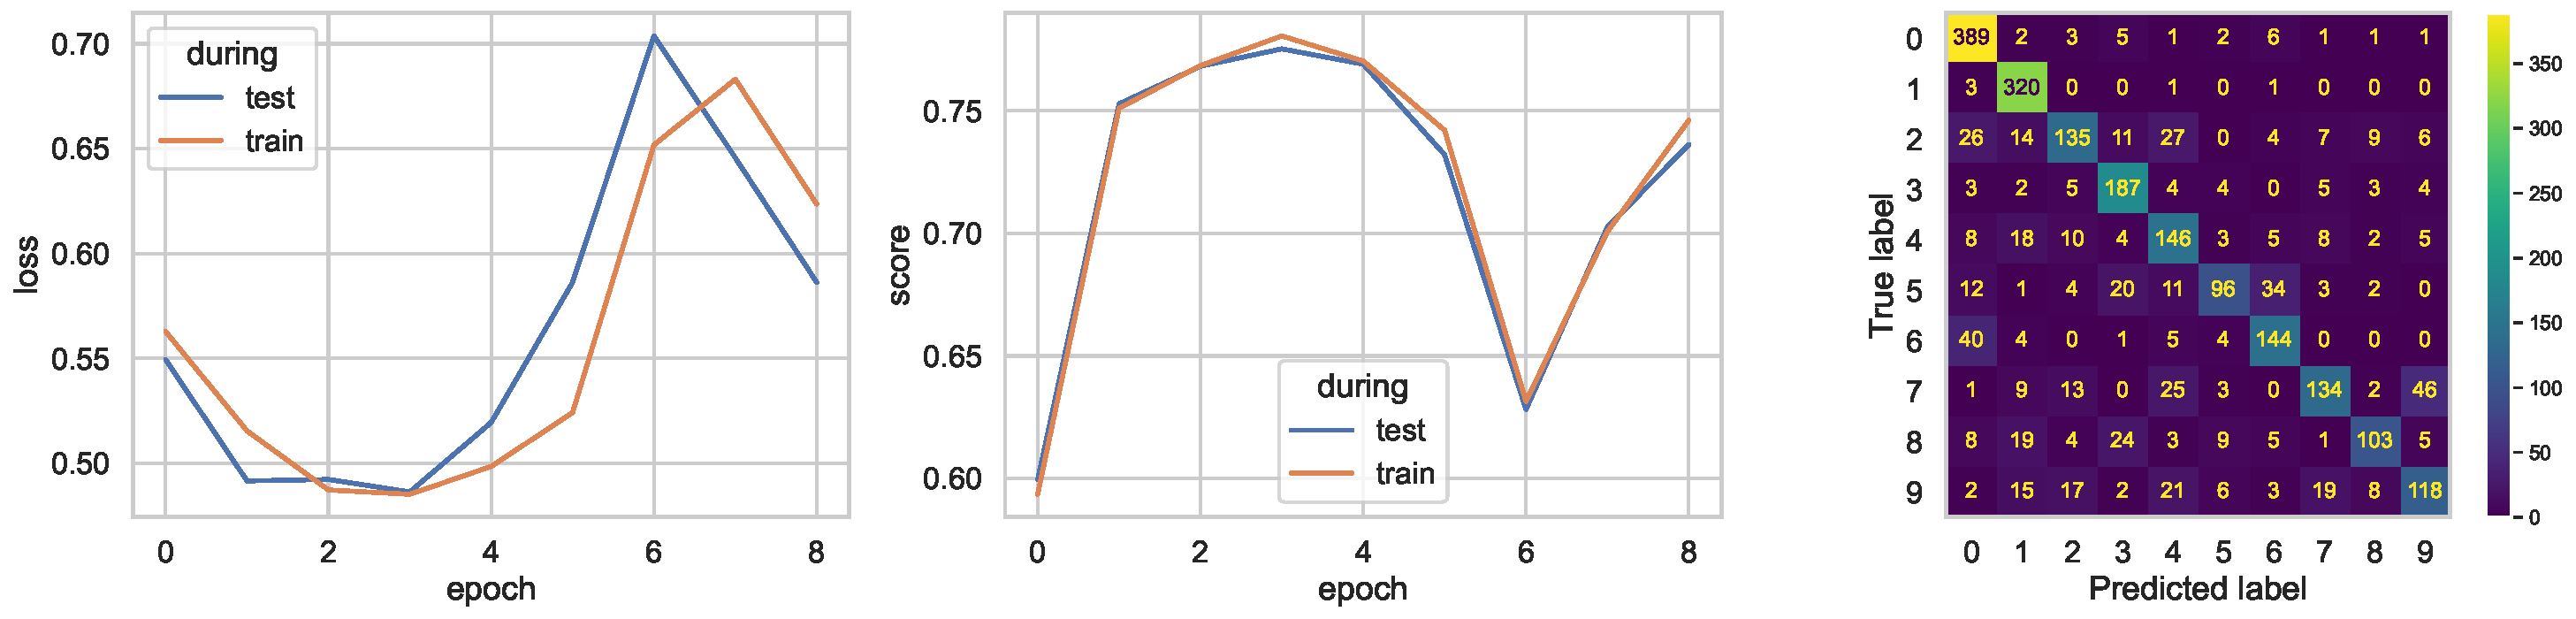
\includegraphics[width=\textwidth]{conv/conv_2layers.pdf}
    \caption{Réseau de neurones convolutionnel à 2 couches}
    \label{fig:conv2layers}
\end{figure}

\paragraph*{Quatre couches convolutionnelles}

\texttt{Conv1D(3, 1, 64, 1)} $\rightarrow$ \texttt{ReLU()} $\rightarrow$ \texttt{MaxPool1D(8, 2)} $\rightarrow$
\texttt{Conv1D(3, 64, 64)} $\rightarrow$ \texttt{ReLU()} $\rightarrow$ \texttt{MaxPool1D(8, 2)} $\rightarrow$
\texttt{Conv1D(3, 64, 64)} $\rightarrow$ \texttt{ReLU()} $\rightarrow$ \texttt{MaxPool1D(8, 2)} $\rightarrow$
\texttt{Conv1D(3, 64, 64)} $\rightarrow$ \texttt{ReLU()} $\rightarrow$ \texttt{MaxPool1D(8, 2)} $\rightarrow$
\texttt{Flatten()} $\rightarrow$
\texttt{Linear(512, 10)}

Les résultats sont sur la figure \ref*{fig:conv4layers} : ici, il parvient mieux à apprendre que le réseau précédent, mais peine à obtenir des performances correctes. On voit par ailleurs que la classe 2 est celle qui est la moins bien classée et est la cause de ce manque de performance : la taille du kernel dans le max pooling est surement trop élevé pour garder un nombre de features significatifs et donc identifier correctement cette classe.

\begin{figure}[htbp]
    \centering
    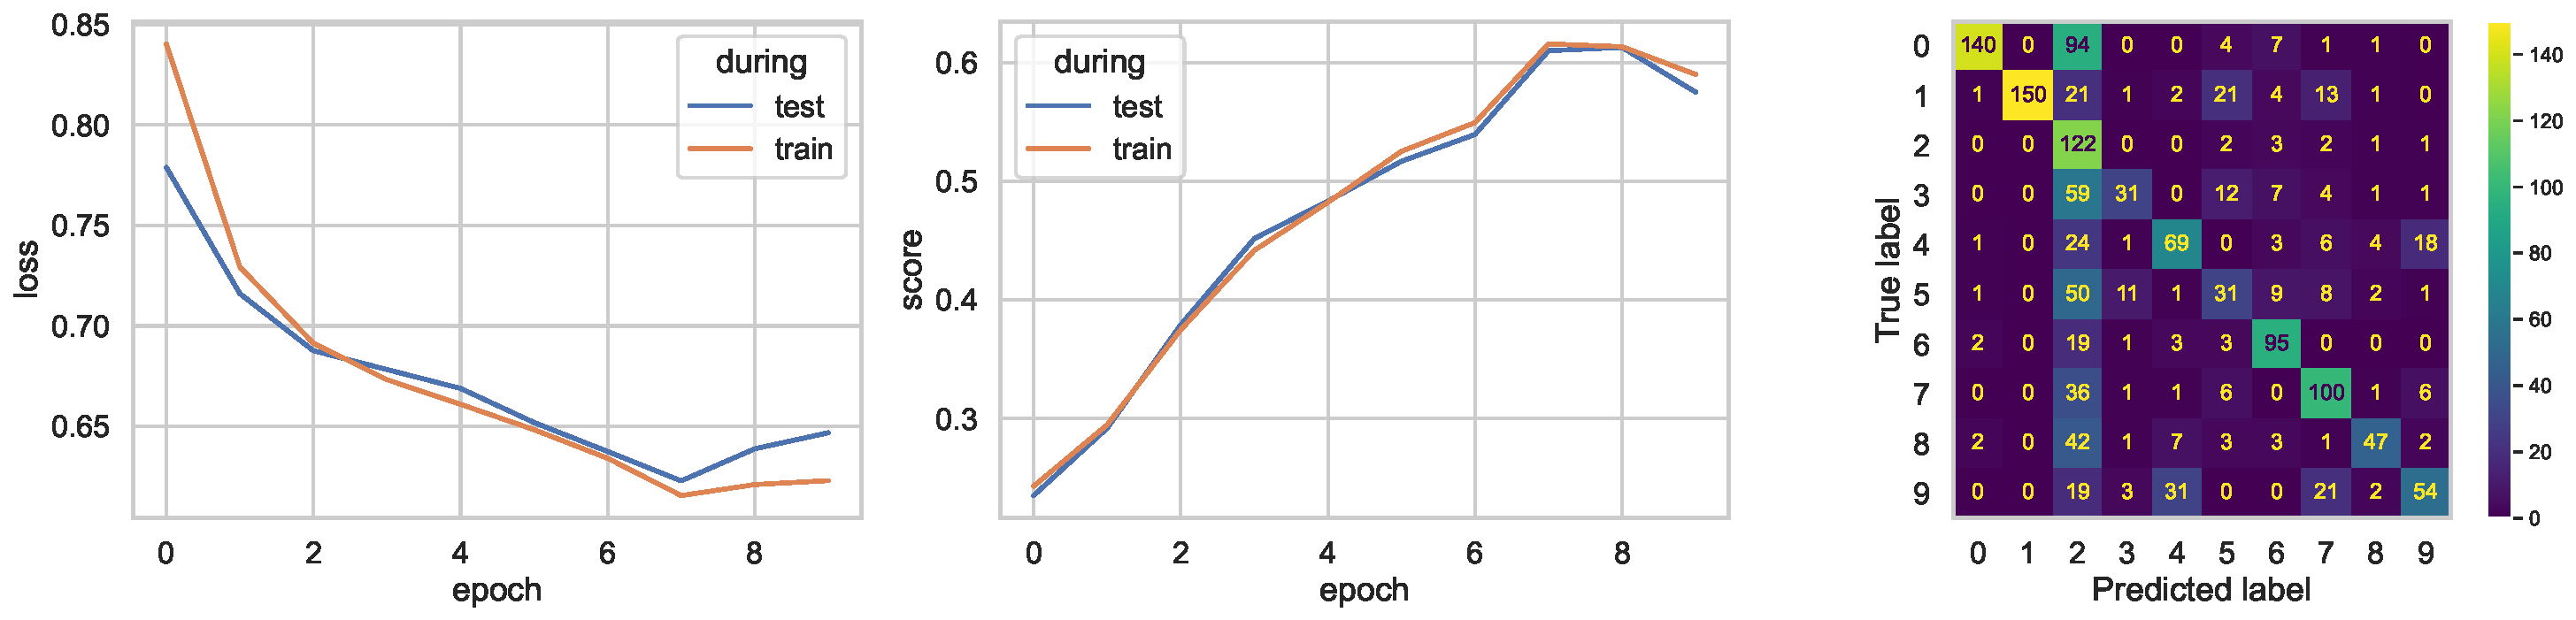
\includegraphics[width=\textwidth]{conv/conv_4layers.pdf}
    \caption{Réseau de neurones convolutionnel à 4 couches}
    \label{fig:conv4layers}
\end{figure}

\subsection{Auto-encodeur}

Nous nous sommes également attelés à des tâches de reconstruction ou de génération de données à l'aide d'architecture encodeur-décodeur (ou auto-encodeur). 

\subsubsection{Reconstruction}

Dans notre cas, on entraîne le modèle à reconstruire les images d'origine à partir de la représentation latente. Pour cela, l'encodeur prend les images d'entrée et les transforme en une représentation latente de dimension réduite. Ensuite, le décodeur prend cette représentation latente et essaie de générer des images qui sont similaires aux images d'origine. L'objectif de cette expérience est de voir comment le modèle est capable de capturer les caractéristiques distinctives des images et de reconstruire des images de qualité. On peut évaluer la performance du modèle en mesurant la différence entre les images reconstruites et les images d'origine.

De plus, l'architecture de l'encodeur-décodeur peut également être utilisée pour générer de nouvelles images similaires à celles du jeu de données MNIST : en fournissant une représentation latente aléatoire au décodeur, il est possible de générer de nouvelles images qui ressemblent aux images du jeu de données.

Nous avons entrainé un auto-encodeur sur les deux jeux de données précédents : (\texttt{USPS} et \texttt{fashion-mnist}). 
\paragraph*{fashion-mnist} 
Ici, trois architecture ont été testé : \begin{enumerate}
    \item \texttt{Linear(784, 64) $\rightarrow$ TanH() $\rightarrow$ décodeur}
    \item \texttt{Linear(784, 256) $\rightarrow$ TanH() $\rightarrow$ Linear(256, 64) $\rightarrow$ TanH() $\rightarrow$ décodeur}
    \item \texttt{Linear(784, 512) $\rightarrow$ TanH() $\rightarrow$ Linear(512, 256) $\rightarrow$ TanH() $\rightarrow$ Linear(256, 128) $\rightarrow$ TanH() $\rightarrow$ Linear(128, 64) $\rightarrow$ TanH() $\rightarrow$ décodeur}
\end{enumerate}
Avec \texttt{décodeur} représentant l'architecture transposé du réseau mais avec une \texttt{Sigmoid()} en sortie. 

Ces trois architectures, plus ou moins complexes, ont toutes mené rapidement à une stagnation du coût d'évalutation durant l'entrainement (voir figure \ref*{fig:lossencoder}). Cette valeur de stagnation varie légérement en fonction de la complexité du réseau. Dans la figure \ref*{fig:reconstruction}, on remarque effectivement que la reconstruction est plus précise en fonction de la complexité du réseau. 

\begin{figure}[htbp]
    \centering
    \includegraphics*[width=.75\textwidth]{loss_encoder_fashion_3_networks.pdf}
    \caption{Valeur de la \texttt{BCELoss()} pour chaque réseau sur 30 epoch}
    \label{fig:lossencoder}
\end{figure}

\begin{figure}[htbp]
    \centering
    \includegraphics*[width=.75\textwidth]{reconstruction_per_network_cplxity.pdf}
    \caption{Exemple de reconstruction en fonction de la complexité du réseau}
    \label{fig:reconstruction}
\end{figure}

Pour le réseau n°1, une étude de l'influence de la fonction d'activation placé avant l'espace latent a été réalisé. Le réseau a donc la forme suivante : \texttt{Linear(784, 64) $\rightarrow$ acc\_fct() $\rightarrow$ décodeur}. Les résultats sont présenté dans la figure \ref*{fig:accfct}. 

\begin{figure}[htbp]
    \centering
    \includegraphics*[width=\textwidth]{encoder_decoder_middle_func_simple_net.pdf}
    \caption{Fonction de cout et reconstruction pour une architecture type réseau n°1}
    \label{fig:accfct}
\end{figure}

On peut voir que le \texttt{Softmax()} et le \texttt{LogSoftmax()} ont des grosses difficultées d'apprentissage. On remarque également que la \texttt{ReLU} apprends beaucoup moins vite que les autres fonction d'activation. 

On s'est aussi amuser à visualiser la reconstruction de l'image au fur et à mesure des époques d'apprentissage dans les figures \ref*{fig:perEpochSimple} et \ref*{fig:perEpochBig}.

\begin{figure}[htbp]
    \centering
    \includegraphics*[width=\textwidth]{reconstruction_per_epoch_simple_model.pdf}
    \caption{Reconstruction par epoch pour le model n°1}
    \label{fig:perEpochSimple}
\end{figure}

\begin{figure}[htbp]
    \centering
    \includegraphics*[width=\textwidth]{reconstruction_per_epoch_big_model.pdf}
    \caption{Reconstruction par epoch pour le model n°3}
    \label{fig:perEpochBig}
\end{figure}

\subsubsection{Organisation de l'espace latent}
Afin de visualiser l'espace latent de 64 dimension, nous avons utiliser la t-SNE afin de le réduire à deux dimensions visualisables. Ce travail a été fait sur les deux jeu de données et sur chacune des séparations entrainement et de test, en utilisant l'auto-encoder le riche en paramètre. Les t-SNE sur le jeu de test sont assez similaire à celle pour le train, nous ne montrerons ici que celle des données d'entrainement. Ces visualisations sont dans les figures \ref*{fig:tsneMnist} et \ref*{fig:tsneUsps}. 

\begin{figure}[htbp]
    \centering
    \includegraphics*[width=.75\textwidth]{tsne_mnist_train_big.pdf}
    \caption{t-SNE sur l'espace latent du modèle n°3 pour \textit{fashion-mnist} en utilisant les données d'entrainement}
    \label{fig:tsneMnist}
\end{figure}

\begin{figure}[htbp]
    \centering
    \includegraphics*[width=.75\textwidth]{tsne_usps_train_big.pdf}
    \caption{t-SNE sur l'espace latent d'un plus gros modèle pour \textit{usps} en utilisant les données d'entrainement}
    \label{fig:tsneUsps}
\end{figure}

Les résultats sont assez intéréssant. En effet on peut voir que les classes zéro, deux, quatre et six n'ont pas de vraiment de cluster, représentant respectivement les T-shirt/top, les Pullover, les mateaux et les chemises. Ces classe étant plus dicifile à distinguer entre elle qu'un pantalon (classe une) ou d'une chaussure (classe 5), elle sont mixé dans l'espace latent.



\subsubsection{Débruitage}

Ici, l'objectif est de reconstruire des images d'origine à partir de versions bruitées, qui est similaire à un travail de reconstruction. Elle montre comment le modèle est capable de supprimer le bruit et de récupérer les informations essentielles des images d'origine. Les trois modèles appris précédemment ont servi à cette tâche.

Avec un bruit gaussien de 20 \%, sur une image de chaque classe. 

Le réseau le plus simple, sur la figure \ref*{fig:reconstruct_noisy_all_small} s'en sort plutôt bien. Bien que l'on perd tout de même en information, notamment au niveau des contours, on parvient à retrouver la forme générale de chaque classe tout en restant fidèle au niveau de gris.

\begin{figure}[htbp]
    \centering
    \includegraphics*[width=\textwidth]{reconstruct_noisy_all_small.pdf}
    \caption{Reconstruction d'une image bruitée de chaque classe pour le réseau n° 1}
    \label{fig:reconstruct_noisy_all_small}
\end{figure}

Le réseau légérement plus complexe, sur la figure \ref*{fig:reconstruct_noisy_all_medium} s'en sort bien également. Il arrive mieux à identifier les contours et les couleurs, pas pour toutes, notamment pour la chaussure de tennis (classe 7), qu'il confond avec des talons. 

\begin{figure}[htbp]
    \centering
    \includegraphics*[width=\textwidth]{reconstruct_noisy_all_medium.pdf}
    \caption{Reconstruction d'une image bruitée de chaque classe pour le réseau n° 2}
    \label{fig:reconstruct_noisy_all_medium}
\end{figure}

Le réseau plus complexe, sur la figure \ref*{fig:reconstruct_noisy_all_big} s'en sort le mieux.

\begin{figure}[htbp]
    \centering
    \includegraphics*[width=\textwidth]{reconstruct_noisy_all_big.pdf}
    \caption{Reconstruction d'une image bruitée de chaque classe pour le réseau n° 3}
    \label{fig:reconstruct_noisy_all_big}
\end{figure}

Sur les figures \ref*{reconstructnoisychaussure}, \ref*{reconstructnoisybag}, \ref*{reconstructnoisypantalon}, \ref*{reconstructnoisycoat}, on fait varier le pourcentage de bruit gaussien ajouté aux données pour comparer la robustesse des modèles. Ainsi, les images débruitées se transforment en tout sauf quelque chose d'original : on reconnait bien souvent une image issue de la classe des vestes ou des t-shirts.

\begin{figure}[htbp]
    \centering
    \includegraphics*[width=\textwidth]{reconstruct_noisy_chaussure.pdf}
    \caption{Reconstruction d'une image bruitée de chaussure}
    \label{fig:reconstructnoisychaussure}
\end{figure}

\begin{figure}[htbp]
    \centering
    \includegraphics*[width=\textwidth]{reconstruct_noisy_sac.pdf}
    \caption{Reconstruction d'une image bruitée de sac}
    \label{fig:reconstructnoisybag}
\end{figure}


\begin{figure}[htbp]
    \centering
    \includegraphics*[width=\textwidth]{reconstruct_noisy_pantalon.pdf}
    \caption{Reconstruction d'une image bruitée de pantalon}
    \label{fig:reconstructnoisypantalon}
\end{figure}


\begin{figure}[htbp]
    \centering
    \includegraphics*[width=\textwidth]{reconstruct_noisy_coat.pdf}
    \caption{Reconstruction d'une image bruitée de manteau}
    \label{fig:reconstructnoisycoat}
\end{figure}


Une grosse amélioration de l'auto-encodeur peut se faire avec des réseaux de neurones convolutionnels mais requièrent des couches de convolutions transposées, qui "déconvolutionnent" des données, ou encore des fonctions d'upsampling. Cela serait également beaucoup plus simple avec une convolution en 2D. Nous avons tenté, en vain, d'utiliser un auto-encodeur avec une architecture ressemblant à : \texttt{Conv1D(3, 1, 32)} $\rightarrow$ {ReLU()} $\rightarrow$ \texttt{MaxPool1D(2, 1)} $\rightarrow$ \texttt{Conv1D(3, 32, 16)} $\rightarrow$ \texttt{ReLU()} $\rightarrow$ \texttt{MaxPool1D(2, 1)} $\rightarrow$ \texttt{Conv1D(3, 16, 16)} $\rightarrow$ \texttt{ReLU()} $\rightarrow$ \texttt{Conv1D(2, 16, 32)} $\rightarrow$ \texttt{ReLU()} $\rightarrow$ \texttt{Conv1D(2, stride=2)} $\rightarrow$ \texttt{Sigmoid()}. Le \textit{padding} serait également nécessaire pour garder la taille d'origine des données.


\section{Conclusion}

Transfert de style aurait été cool mais besoin de conv2d et on avait pas le temps mashallah

traduction 

opti gpu et compilation 



\end{document}